\documentclass[10pt,twocolumn,letterpaper]{article}

\usepackage{cvpr}
\usepackage{times}
\usepackage{epsfig}
\usepackage{graphicx}
\usepackage{amsmath}
\usepackage{amssymb}

\def\cvprPaperID{1} % *** Enter the CVPR Paper ID here

\usepackage[breaklinks=true,bookmarks=false]{hyperref}

\cvprfinalcopy % Comment this line and it stop working! :(
\ifcvprfinal\pagestyle{empty}\fi

\def\httilde{\mbox{\tt\raisebox{-.5ex}{\symbol{126}}}}

% Pages are numbered in submission mode, and unnumbered in camera-ready
%\ifcvprfinal\pagestyle{empty}\fi
\setcounter{page}{1}

\graphicspath{ {./images/} } 

\sloppy

%-------------------------------------------------------------------------
%-------------------------------------------------------------------------

\begin{document}

%%%%%%%%% TITLE
\title{Comparison of SegNet and U-Net for Semantic Segmentation}

\author{Felipe Augusto Lima Reis\\
PUC Minas - Pontif\'icia Universidade Cat\'olica de Minas Gerais\\
R. Walter Ianni 255 - Bloco L - Belo Horizonte, MG, Brasil\\
{\tt\small falreis@sga.pucminas.br}
}

\maketitle
%\thispagestyle{empty}

%%%%%%%%% ABSTRACT
%Briefly describe your problem, approach, and key results. Should be no more than 300 words.

\begin{abstract}
    Image segmentation refers to the partition of an image into a set of regions to cover it, to represent a meaningful area. Before the use of deep neural networks, the best-performing methods mostly was made using hand engineered features \cite{SEGNET}. This paper will evaluate two Deep Neural Networks for semantic segmentation: SegNet and U-Net. These DNNs are both ``fully convolutional'' networks that output a result with the same size as the input. The models are trained and tested using KITTI Road Dataset. The results were also evaluated using KITTI Dataset Toolkit. The tests showed that SegNet had a better performance in image segmentation than U-Net. U-Net, however, was easier to train, smaller and provide faster results than SegNet.
\end{abstract}

%%%%%%%%% BODY TEXT


%##################################################################################################
\section{Introduction} \label{introduction}
%Describe the problem you are working on, why it's important, and an overview of your results

Image segmentation refers to the partition of an image into a set of regions to cover it, to represent meaningful areas \cite{DOMINGUEZ}. The goal is to simplify and/or change the representation of an image into something that is more meaningful and easier to analyze \cite{AHMED_SARMA}.

Segmentation has two main objectives: the first one is to decompose the image into parts for further analysis and the second one is to perform a change of representation \cite{DOMINGUEZ}. Also, segmentation must follow some characteristics to identify regions, as it follows:

\begin{itemize}
 \item Regions of an image segmentation should be uniform and homogeneous with respect to some characteristic, such as gray level, color, or texture \cite{DOMINGUEZ};
 \item Region interiors should be simple and without many small holes \cite{DOMINGUEZ};
 \item Adjacent regions of a segmentation should have significantly different values with respect to the characteristic on which they are uniform \cite{DOMINGUEZ};
 \item Boundaries of each segment should be smooth, not ragged, and should be spatially accurate \cite{DOMINGUEZ}.
\end{itemize}

Semantic pixel-wise segmentation is an active topic of research \cite{SEGNET}. Before the use of deep neural networks, the best-performing methods mostly was made using hand engineered features \cite{SEGNET}. The success of deep convolutional neural networks for object classification led researchers to use these techniques to learn new capabilities, such as segmentation \cite{SEGNET}.

This paper will evaluate two different Deep Neural Networks for semantic segmentation and compare the results over Kitti Road Dataset \cite{KITTI}. The chosen neural networks are SegNet \cite{SEGNET} and U-Net \cite{UNET}.

The organization of this paper is as follows. In the next Section we show related works to this paper. Section \ref{sec:data} contains information about the dataset used in this work as other datasets used previously to start the project. Section \ref{sec:methods} explains the methods used to develop this project, Section \ref{sec:experiments} describe the experiments and shows the results and Section \ref{sec:conclusion} concludes this paper and gives some final considerations and ideas for future works.


%##################################################################################################
\section{Related Work} \label{sec:related_work}
%Discuss published work that relates to your project. How is your approach similar or different from others?

Our approach follows the recent successes of deep neural networks for image classification \cite{VGGNET} \cite{AHMED_SARMA}, transfer learning \cite{PRATT} \cite{WEISS2016} and semantic segmentation \cite{SEGNET} \cite{UNET} \cite{FULLY_CONVOLU}. Also, the paper follow classical methods for segmentation \cite{WATERSHEDS} \cite{SLIC} \cite{LATTICES} \cite{FELZENSZWALB}, developed before the usage of neural nets.

\subsection{Superpixels} \label{ssec:superpixels}

Before the use of deep neural networks, the best-performing methods to segmentation mostly was made using hand engineered features \cite{SEGNET}. Some common features used pixels as basic units of processing \cite{WANG201728}. Superpixels are the result of perceptual grouping of pixels \cite{WANG201728}. Superpixels produces segmentation of coarse granulation, that can be call oversegmentation \cite{WANG201728}. Superpixel segmentation showed to be a useful pre-processing step in many computer vision applications \cite{WANG201728}.

There has been a lot of research on superpixels since the term has been established \cite{WANG201728}. In particular, various algorithms for superpixel segmentations have been proposed. Algorithms for generating superpixels can be broadly categorized as either graph-based or gradient ascent methods \cite{SLIC}, as described below:

\begin{itemize}
 \item \textit{Graph-based algorithms}: Graph-based approaches to superpixel generation treat each pixel as a node in a graph. Edge weights between two nodes are proportional to the similarity between neighboring pixels. Superpixels are created by minimizing a cost function defined over the graph \cite{SLIC}. Example of this category are the \textit{Efficient Graph-Based Image Segmentation} (EGB) algorithm \cite{FELZENSZWALB} and the \textit{Superpixels Lattices} \cite{LATTICES};
 \item \textit{Gradient-ascent-based algorithms}: Starting from a rough initial clustering of pixels, gradient ascent methods iteratively refine the clusters until some convergence criterion is met to form superpixels \cite{SLIC}. In this set, its possible to cite \textit{watersheds} algorithms \cite{WATERSHEDS} and the \textit{SLIC} algorithm \cite{SLIC};
\end{itemize}

%-------------------------------------------------------------------------
\subsection{Fully Convolutional Networks} \label{ssec:fully_conv}

Each layer of data in a convnet is a three-dimensional array of size $h \times w \times d$, where $h$ and $w$ are spatial dimensions, and $d$ is the feature or channel dimension \cite{FULLY_CONVOLU}. The first layer is the image, with pixel size $h \times w$, and $d$ color channels \cite{FULLY_CONVOLU}. Locations in higher layers correspond to the locations in the image they are path-connected to, which are called their receptive fields \cite{FULLY_CONVOLU}.

Convnets are built on translation invariance. Their basic components (convolution, pooling, and activation functions) operate on local input regions, and depend only on relative spatial coordinates \cite{FULLY_CONVOLU}. While a general deep net computes a general nonlinear function, a net with only layers of this form computes a
nonlinear filter, which we call a deep filter or fully convolutional network. An FCN naturally operates on an input of any size, and produces an output of corresponding (possibly resampled) spatial dimensions \cite{FULLY_CONVOLU}.

%-------------------------------------------------------------------------
\subsubsection{SegNet} \label{sssec:segnet}

SegNet is a deep encoder-decoder architecture for multi-class pixelwise segmentation \cite{SEGNET}. The SegNet architecture consists of a sequence of non-linear processing layers (encoders) and a corresponding set of decoders followed by a pixel-wise classifier \cite{SEGNET} \cite{SEGNET_WEBSITE}. Typically, each encoder consists of one or more convolutional layers with batch normalization and a ReLU non-linearity, followed by non-overlapping max-pooling and sub-sampling \cite{SEGNET} \cite{SEGNET_WEBSITE}. The sparse encoding due to the pooling process is upsampled in the decoder using the max-pooling indices in the encoding sequence \cite{SEGNET} \cite{SEGNET_WEBSITE}. Figure \ref{fig:segnet} presents the architecture of SegNet.

\begin{figure}[ht]
  \centering
  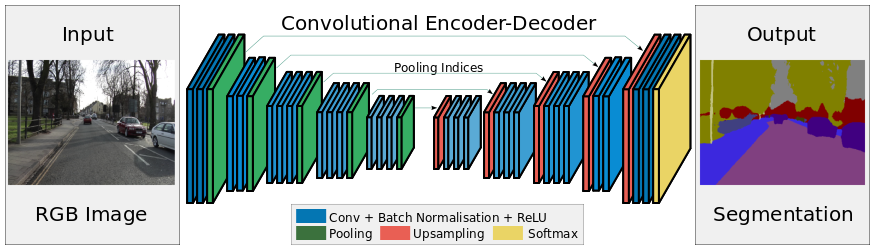
\includegraphics[width=0.48\textwidth]{segnet.png}
  \caption{SegNet architecture. \textit{Image adapted from SegNet project website} \cite{SEGNET_WEBSITE} \cite{SEGNET}}
  \label{fig:segnet}
\end{figure}

%-------------------------------------------------------------------------
\subsubsection{U-Net} \label{sssec:unet}

U-Net is a Convolutional Networks for Biomedical Image Segmentation \cite{UNET} \cite{UNET_WEBSITE}. Although U-Net was developed for biomedical image segmentation, its architecture can be trained to segment other types of image.

U-Net architecture consists of the repeated application of two $3 \times 3$ convolutions, each followed by a rectified linear unit (ReLU) and a $2 \times 2$ max pooling operation with stride 2 for downsampling \cite{UNET}. Every step in the expansive path consists of an upsampling of the feature map followed by a $2 \times 2$ convolution, a concatenation with the correspondingly cropped feature map from the contracting path, and two $3 \times 3$ convolutions, each followed by a ReLU \cite{UNET}. At the final layer a $1 \times 1$ convolution is used. In total the network has 23 convolutional layers \cite{UNET}. Figure \ref{fig:unet} presents the  architecture of U-Net.

\begin{figure}[ht]
  \centering
  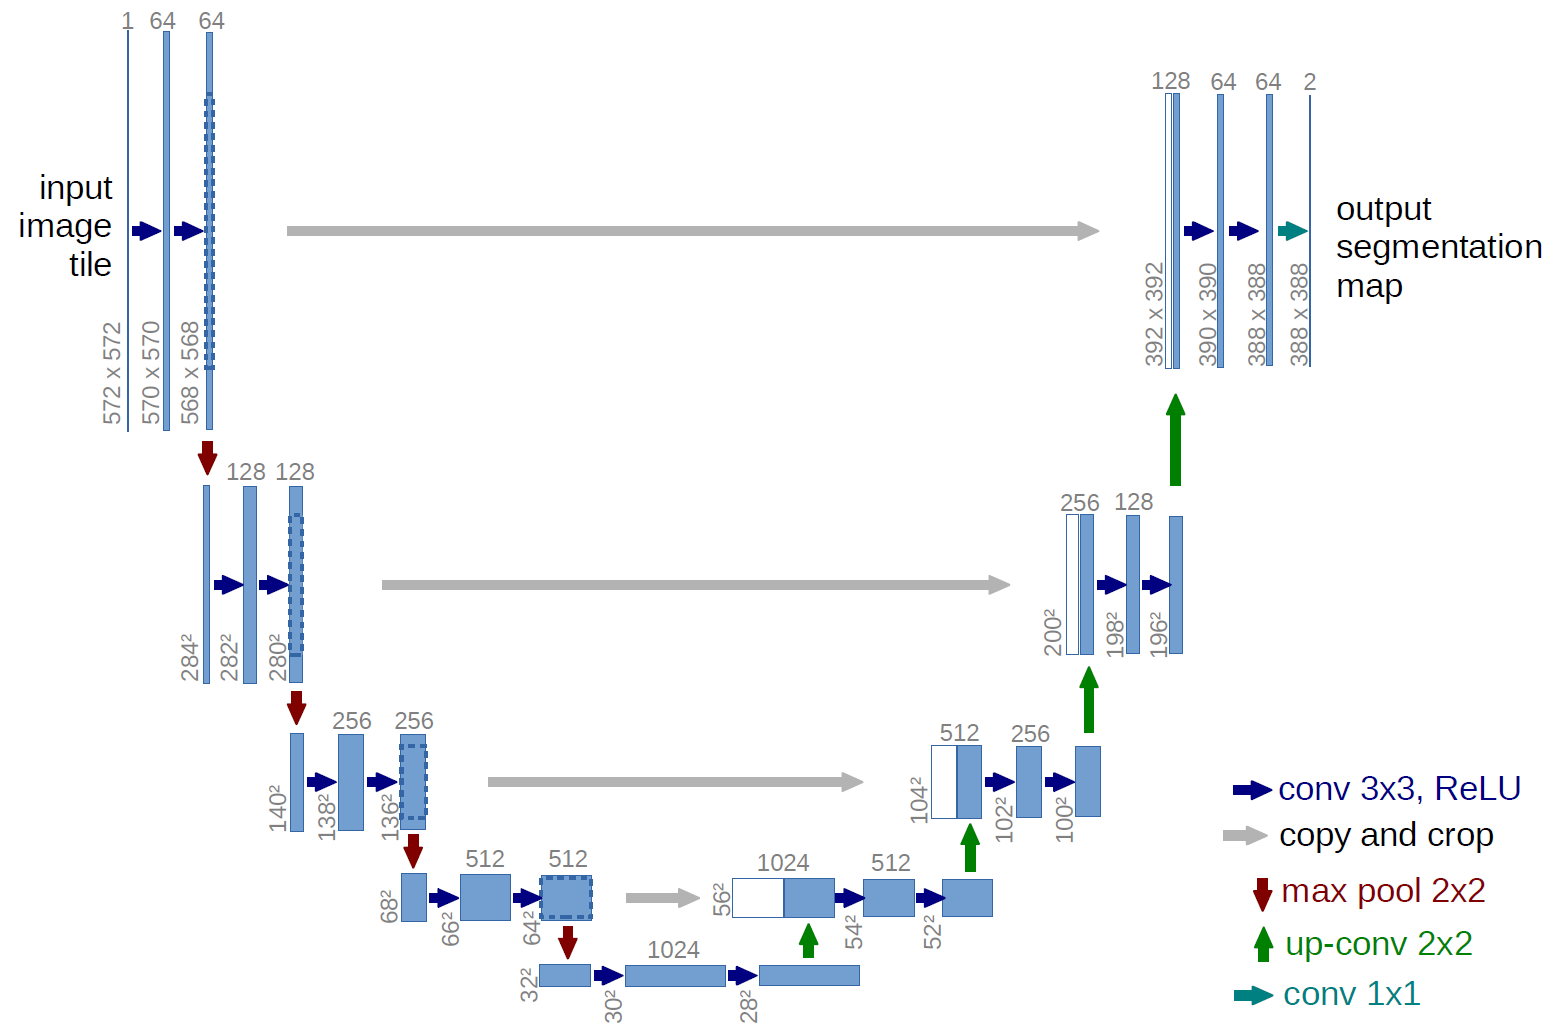
\includegraphics[width=0.48\textwidth]{unet.png}
  \caption{U-Net architecture. \textit{Image adapted from U-Net project website} \cite{UNET_WEBSITE} \cite{UNET}}
  \label{fig:unet}
\end{figure}


%##################################################################################################
\section{Data} \label{sec:data}

%Describe the data you are working with for your project. What type of data is it? Where did it come from? How much data are you working with? Did you have to do any preprocessing, filtering, or other special treatment to use this data in your project?

KITTI Vision Benchmarking Suite is an project of Karlsruhe Institute of Technology and Toyota Technological Institute at Chicago to provide an real-world computer vision benchmark for autonomous driving platform Annieway \cite{KITTI_FULL} \cite{KITTI_WEBSITE}. KITTI contains benchmarks and datasets for the following area of interests: stereo, optical flow, visual odometry, 3D object detection and 3D tracking \cite{KITTI_WEBSITE}.

One of the benchmark in KITTI suite is the Road/Lane Dataset Evaluation \cite{KITTI}. The road and lane estimation benchmark consists of 289 training and 290 test images, in four different categories of road scenes \cite{KITTI}:

\begin{itemize}
 \item uu - urban unmarked (98 training images and 100 test images) \cite{KITTI};
 \item um - urban marked (95 training images and 96 test images) \cite{KITTI};
 \item umm - urban multiple marked lanes (96 training images and 94 test images) \cite{KITTI};
 \item urban - combination of the three above \cite{KITTI}.
\end{itemize}

Ground truth has been generated by manual annotation of the images and is available for two different road terrain types: road - the road area (the composition of all lanes), and lane (the ego-lane, the lane the vehicle is currently driving on) \cite{KITTI} \cite{KITTI_WEBSITE}. Ground truth is provided for training images only \cite{KITTI}. 

As the dataset do not provide test groundtruth, the results must be evaluated using a benchmarking tool provided with the dataset \cite{KITTI_WEBSITE}. This tool  performs road and lane estimation in the bird's-eye-view space \cite{KITTI} \cite{KITTI_WEBSITE}. The metrics used are Maximum F1-measure, Average precision as used in PASCAL VOC challenges, Precision, Recall, False Positive Rate, False Negative Rate, F1 score and Hit Rate \cite{KITTI} \cite{KITTI_WEBSITE}.

%-------------------------------------------------------------------------
\subsection{Other Evaluated Datasets} \label{ssec:other_datasets}

The two datasets presented in this section were evaluted also for this paper, but, the final results does not contains both. The reasons to prefer KITTI over CamVid and BSDS500 datasets are available in Sections \ref{sec:experiments} and \ref{sec:conclusion}.

%-------------------------------------------------------------------------
\subsubsection{CamVid Dataset} \label{sssec:camvid_datasets}

The Cambridge-driving Labeled Video Database (CamVid) is the first collection of videos with object class semantic labels, complete with metadata \cite{CAMVID}. The database provides ground truth labels that associate each pixel with one of 32 semantic classes \cite{CAMVID}. The database addresses the need for experimental data to quantitatively evaluate emerging algorithms \cite{CAMVID}.

%-------------------------------------------------------------------------
\subsubsection{BSDS500 Dataset} \label{sssec:bsds_dataset}

Berkeley Segmentation Data Set contains 500 natural images and its respective ground-truths, annotated by humans \cite{BSDS500}. The images are explicitly separated into disjoint train, validation and test subsets \cite{BSDS500}.

To evaluate the quality of the segmentation methods, BSDS500 provides a benchmarking tool \cite{BSDS500}. BSDS500 dataset uses the Precision and Recall Method to evaluate the results \cite{BSDS500}.


%##################################################################################################
\section{Methods} \label{sec:methods}

%Discuss your approach for solving the problems that you set up in the introduction. Why is your approach the right thing to do? Did you consider alternative approaches? You should demonstrate that you have applied ideas and skills built up during the quarter to tackling your problem of choice. It may be helpful to include figures, diagrams, or tables to describe your method or compare it with other methods.

%-------------------------------------------------------------------------
\subsection{Transfer Learning} \label{ssec:transfer_learning}

Transfer learning is a technique in machine learning that stores knowledge gained while solving one problem, adapt and apply it to a different but related problem. As the growing of neural networks usage, it becomes reasonable to seek out methods that avoid ``reinventing the wheel'', and instead are able to build on previously trained networks' results \cite{PRATT} \cite{WEISS2016}.

As the images of KITTI Dataset are really different from any other tested images, the usage of transfer learning needs to shrink some parts of the image and grow other, defforming a lot the original image. Then, this work started trying to use transfer learning, but decided set aside the results.

%-------------------------------------------------------------------------
\subsection{Data Augmentation} \label{ssec:data_augmentation}

Data augmentation consists of a range of transformations that can be applied to the dataset to increase the number of data with the target of improving the accuracy and robustness of classifiers \cite{AUGM_ADAPT}. The problem with small datasets is that models trained with them do not generalize well \cite{AUGM_DEEP}.

Data augmentation also can act as a regularizer in preventing overfitting in neural networks and improve performance in imbalanced class problems \cite{DATA_AUGM}. According to Wong et al. \cite{DATA_AUGM}, data augmentation is better to perform in data-space instead of feature-space, as long as label preserving transforms are known \cite{DATA_AUGM}.

To provide data augmentation, the images and the ground-truth will be rotated 12 times, 30 degrees each. Also, the images will be flipped and rotated 12 times each. Then, each image will transform into 24 possible images. Then, 200 images for the training set will become 4800 training images and the validation set will contains 2400 images. The number of images is not too big but can help the DNN predict with more accuracy.

%-------------------------------------------------------------------------
\subsection{Other Data Augmentation} \label{ssec:data_augmentation}

Mostrar informações e imagens sobre o problema de virar a imagem de cabeça para baixo.

%-------------------------------------------------------------------------
\subsection{SegNet Model} \label{ssec:segnet_model}

\ref{fig:segnet_model}

\begin{figure}[ht]
  \centering
  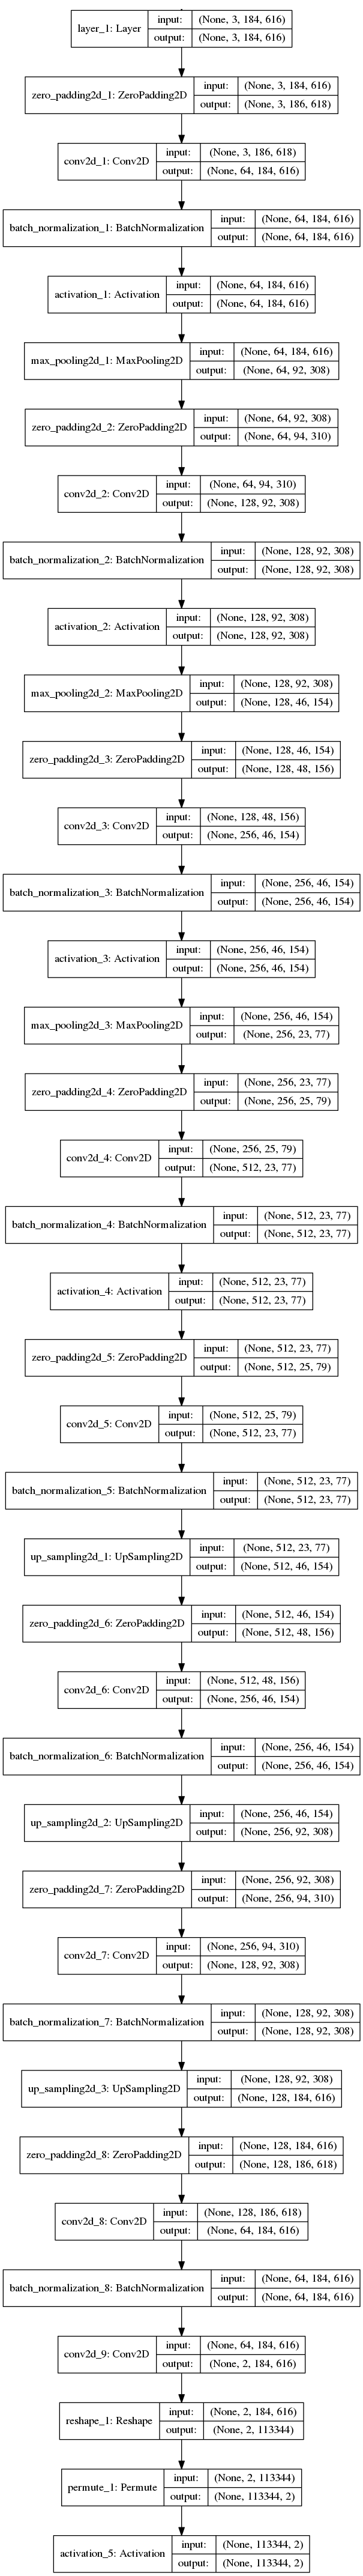
\includegraphics[width=0.19\textwidth]{kitti_segnet_plot.png}
  \caption{SegNet architecture for KITTI Road/Lane Dataset.}
  \label{fig:segnet_model}
\end{figure}

%-------------------------------------------------------------------------
\subsection{U-Net Model} \label{ssec:unet_model}

\ref{fig:unet_model}

\begin{figure}[ht]
  \centering
  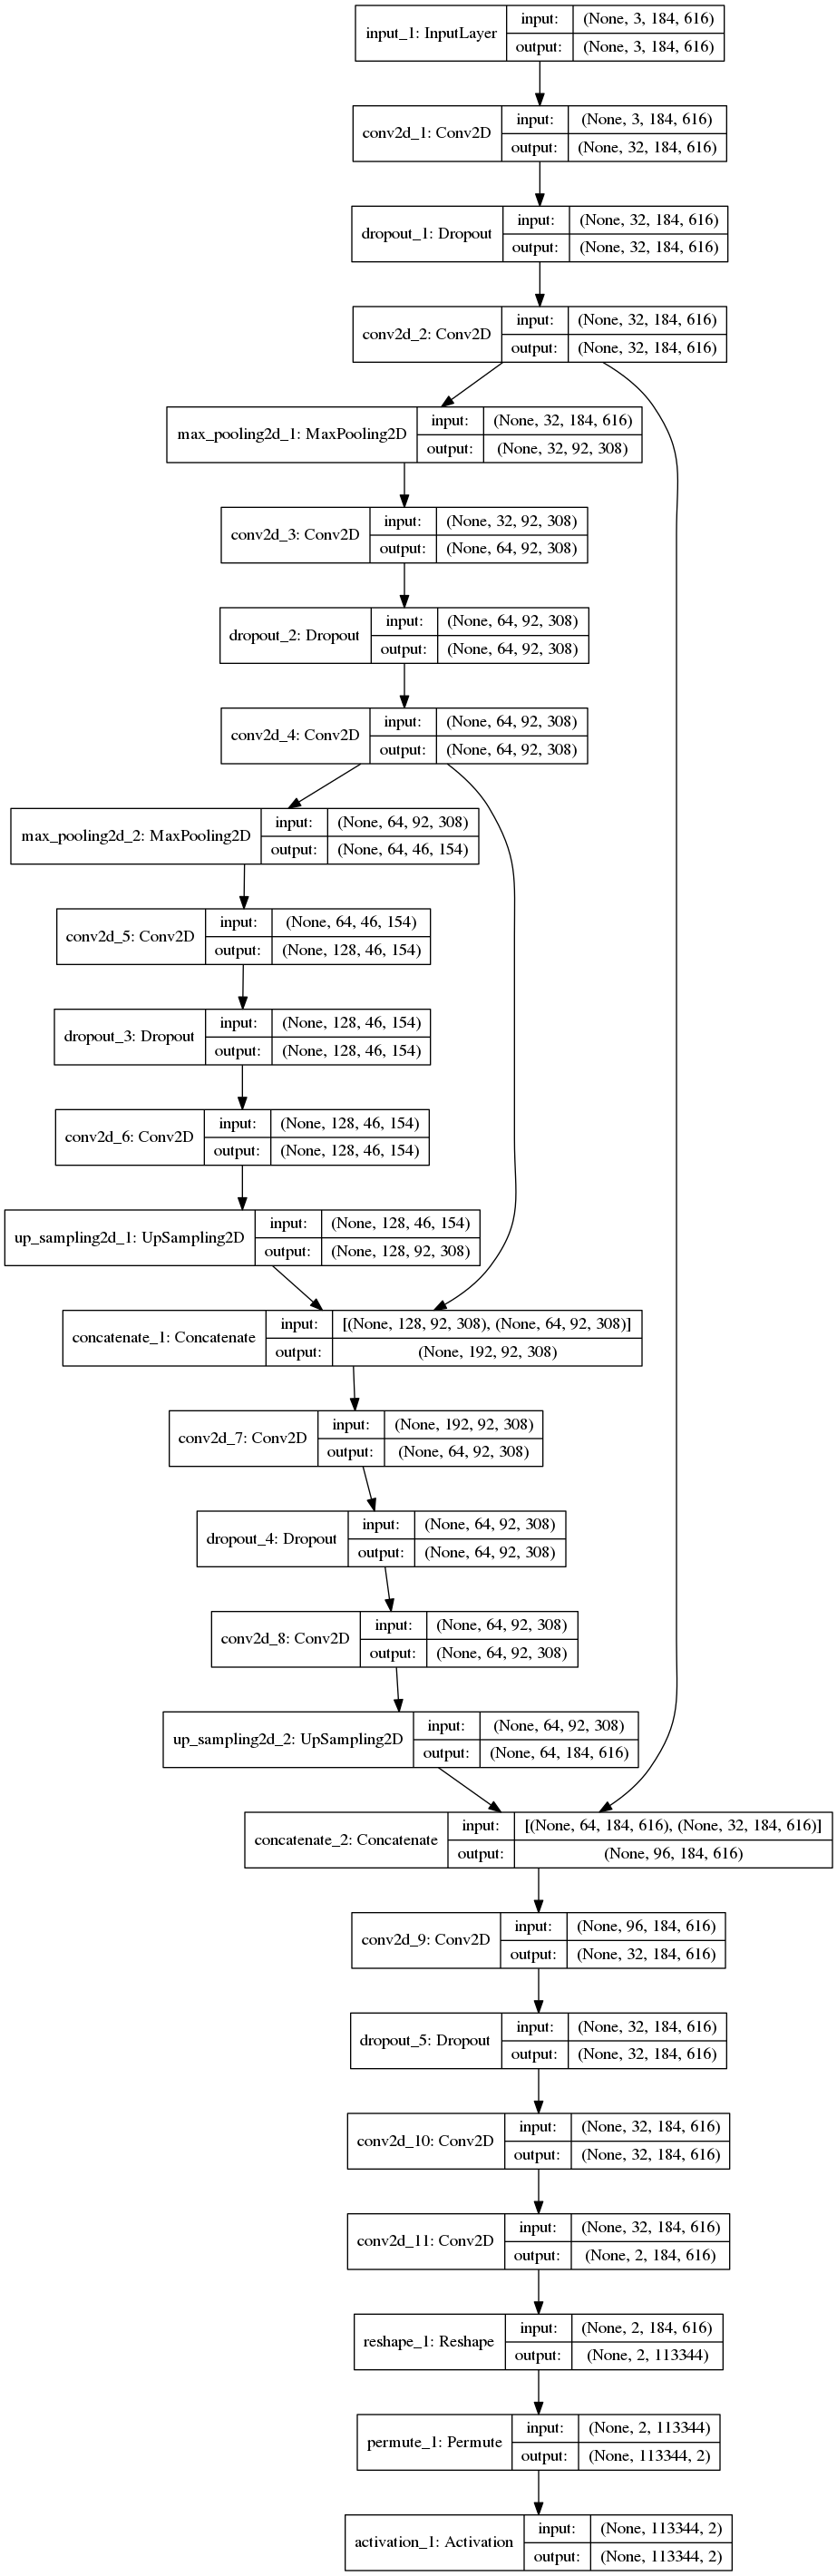
\includegraphics[width=0.45\textwidth]{kitti_unet_plot.png}
  \caption{U-Net architecture for KITTI Road/Lane Dataset.}
  \label{fig:unet_model}
\end{figure}

%##################################################################################################
\section{Experiments} \label{sec:experiments}

%Discuss the experiments that you performed to demonstrate that your approach solves the problem. The exact experiments will vary depending on the project, but you might compare with previously published methods, perform an ablation study to determine the impact of various components of your system, experiment with different hyperparameters or architectural choices, use visualization techniques to gain insight into how your model works, discuss common failure modes of your model, etc. You should include graphs, tables, or other figures to illustrate your experimental results.

\subsection{Environment} \label{ssec:environment}

The tests described in this section were performed in a Amazon AWS \cite{AMAZON_WEBSITE} \textit{g2.2xlarge} Instance. The instance contains 8 vCPUs of Intel Corporation 440FX CPU and 15GB RAM memory. Also, contains a NVIDIA Corporation GK104GL [GRID K520] GPU, with 4096 MB x2 GDDR5 memory. The custom configuration were a 100GB SSD storage capacity with a pre-configured Amazon Linux OS (Deep Learning AMI Version 12.0 - \textit{ami-f6a94495}).


The pre-trained VGG-16 will be provided by Keras, a Python Deep Learning Library \cite{KERAS}. Keras is a high-level neural networks API of running on top of TensorFlow \cite{TENSORFLOW}, CNTK \cite{CNTK}, or Theano \cite{THEANO} \cite{KERAS}.

%##################################################################################################
\section{Conclusion} \label{sec:conclusion}

%Summarize your key results - what have you learned? Suggest ideas for future extensions or new applications of your ideas.

%-------------------------------------------------------------------------

{\small
\bibliographystyle{ieee}
\bibliography{egbib}
}

\end{document}
